Toutes les études réalisées dans cette section reposent sur la même méthodologie. Les facteurs de vue théoriques sont établis à partir de la littérature \cite{Howell} et sont disponibles en Annexe \ref{anx:fv}. 

Afin d’évaluer quantitativement la qualité des matrices de facteurs de vue obtenues par le code de Monte Carlo Ray Tracing, celles-ci sont comparées à une matrice de référence $F^{\mathrm{ref}}$. L’écart est mesuré via une erreur quadratique moyenne relative (Relative Root Mean Square Error, RRMSE), définie à partir de l’erreur relative élémentaire.

Pour chaque coefficient non négligeable de la matrice de référence, l’erreur relative est définie par :

\begin{equation}
\varepsilon_{ij} =
\frac{
F_{ij}^{\mathrm{calc}} - F_{ij}^{\mathrm{ref}}
}{
F_{ij}^{\mathrm{ref}}
}.
\end{equation}

Afin d’éviter les divisions par des valeurs nulles ou numériquement négligeables, seuls les coefficients vérifiant :

\begin{equation}
\left|F_{ij}^{\mathrm{ref}}\right| > \varepsilon_{\mathrm{th}},
\qquad \text{avec } \varepsilon_{\mathrm{th}} = 10^{-15},
\end{equation}

sont retenus dans le calcul. L’ensemble des indices satisfaisant cette condition est noté $\Omega$.

La métrique globale est ensuite définie comme la racine de la moyenne des carrés des erreurs relatives :

\begin{equation}
\mathrm{RRMSE}
=
\sqrt{
\frac{1}{|\Omega|}
\sum_{(i,j)\in \Omega}
\varepsilon_{ij}^{2}
}.
\end{equation}

Cette grandeur fournit une mesure globale, sans dimension, de l’écart entre la matrice calculée et la matrice de référence. Une valeur nulle correspond à une concordance exacte, tandis qu’une augmentation de cette métrique traduit une dégradation progressive de l’accord entre les deux solutions. Cette grandeur est utilisée par la suite pour analyser la convergence et la qualité des résultats en fonction des paramètres de simulation.

\subsection{Simulation MCRT en 3D}

\begin{figure}[H]
\centering

\begin{minipage}{0.45\textwidth}
\centering

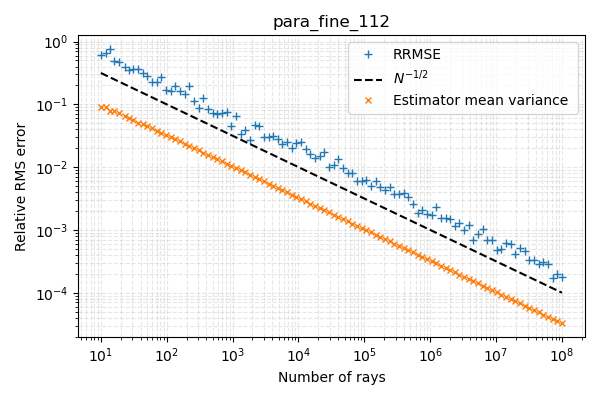
\includegraphics[width = 1\linewidth]{PICTURES/c2/VERIF/rms_convergence_para_fine_112.png}
\small\textbf{(a) Cas d'un parallélépipède}
\end{minipage}
\hfill
\begin{minipage}{0.45\textwidth}
\centering
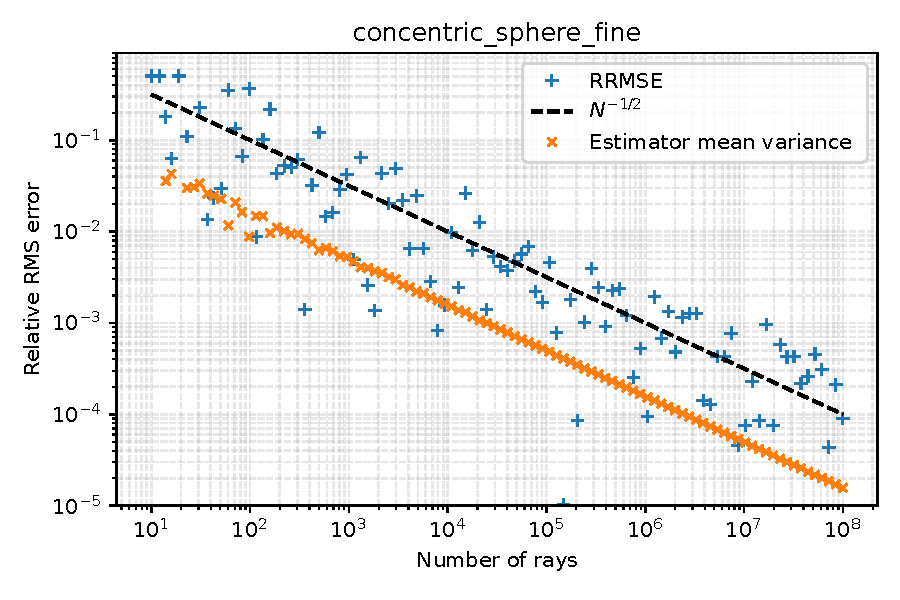
\includegraphics[width = 1\linewidth]{PICTURES/c2/VERIF/convergence_cs_f.pdf}


\small\textbf{(b) Cas de deux sphères concentriques}
\end{minipage}

\caption{Convergence des facteurs de vue pour des géométries en 3D.}
\label{fig:verif3D}

\end{figure}
\subsection{Simulation MCRT avec des géométries 2D}
\label{part:2Dcomp}

\begin{figure}[H]
\centering

\begin{minipage}{0.45\textwidth}
\centering

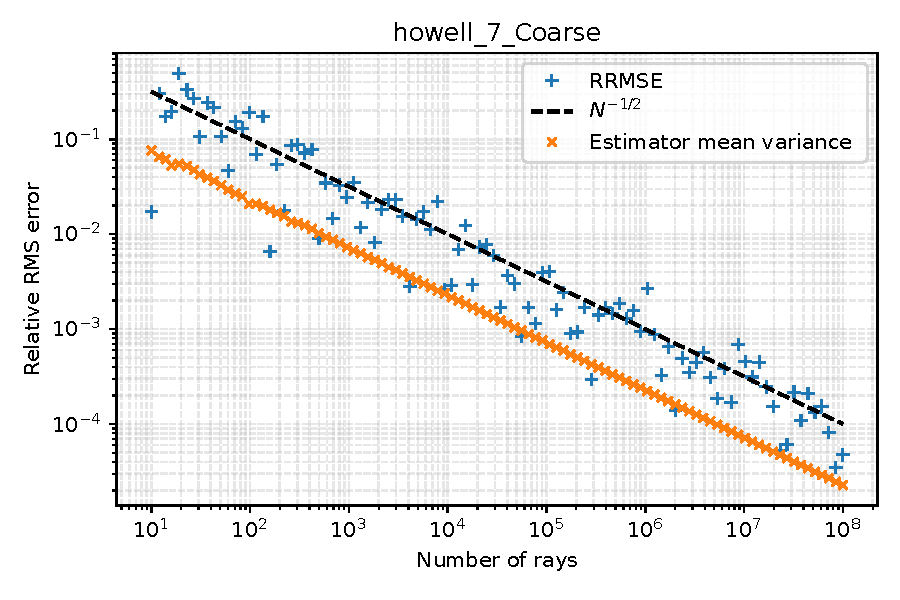
\includegraphics[width = 1\linewidth]{PICTURES/c2/VERIF/convergence_h7.pdf}
\small\textbf{(a) Cas de deux arrêtes adjacentes d'un carré}
\end{minipage}
\hfill
\begin{minipage}{0.45\textwidth}
\centering
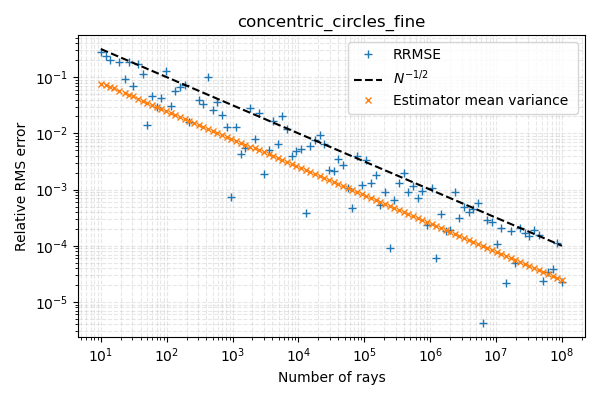
\includegraphics[width = 1\linewidth]{PICTURES/c2/VERIF/convergence_cc_fine.png}


\small\textbf{(b) Cas de deux cercles concentriques}
\end{minipage}

\caption{Convergence des facteurs de vue pour des géométries en 2D.}
\label{fig:verif3D}

\end{figure}







\subsection{Simulation MCRT avec des faces miroires}
\begin{figure}[H]
\centering

\begin{minipage}{0.45\textwidth}
\centering

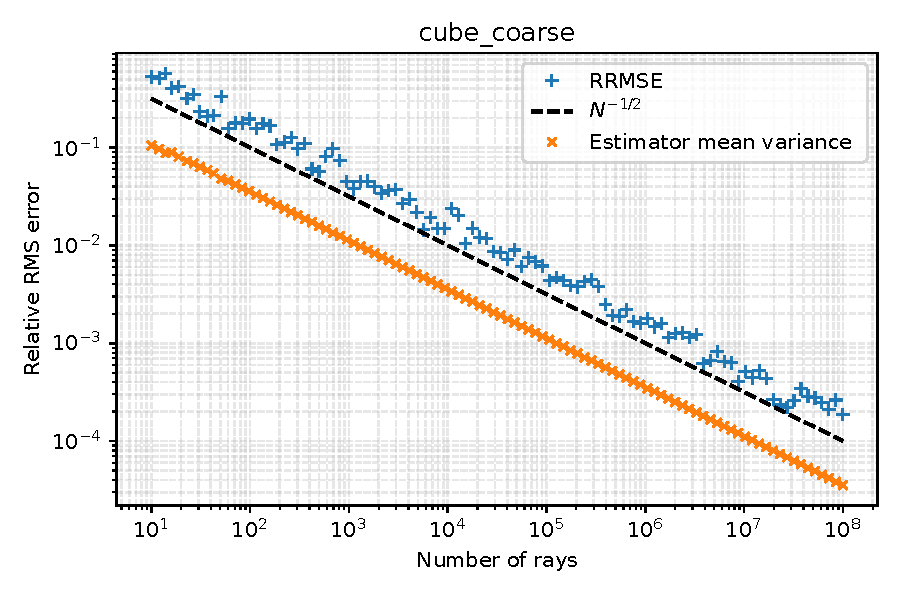
\includegraphics[width = 1\linewidth]{PICTURES/c2/VERIF/convergence_cube_sym_coarse.pdf}
\small\textbf{(a) Cas d'un cube avec une face miroire}
\end{minipage}
\hfill
\begin{minipage}{0.45\textwidth}
\centering
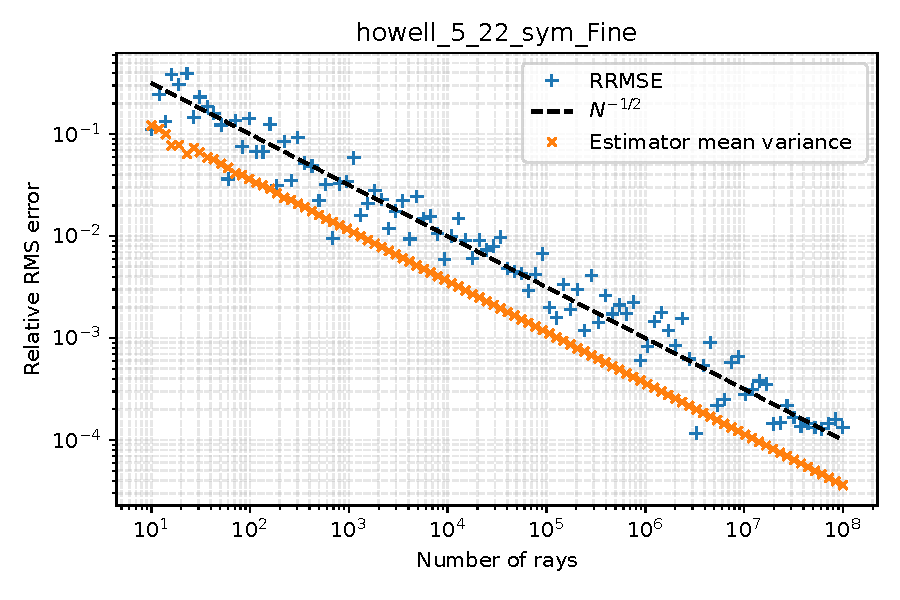
\includegraphics[width = 1\linewidth]{PICTURES/c2/VERIF/convergence_h5_22_sym_Fine.pdf}


\small\textbf{(b) Cas d'une rangée infinie de cercle}
\end{minipage}

\caption{Convergence des facteurs de vue pour des géométries avec faces réflectives.}
\label{fig:verif3Dmiror}

\end{figure}

